%% -----------------------------------------------------------------------------

A type-level mutation is {\em interesting\/} (1) if, upon removal of the type
annotations, running the program raises a run-time error, (2) whose stack trace
contains source locations from at least three modules, and (3) if this happens
in all of the to-be-evaluated semantics. An interesting mutation represents a
{\em debugging scenario\/} that supplies the rational programmer with
information.

Here is the rationale for these three conditions:
\begin{enumerate}

\item By definition, an impedance mismatch is a class between type ascription of
one module to another module's exports. Hence, type checking fails for an
interesting mutant module, and removing the types from this mutant module
creates an impedance mismatch between it and the modules that import it,
directly or indirectly. This impedance mismatch is of interest if, and only if,
running the program leads to an exception---otherwise it goes unobserved and
cannot be debugged.

\item If the evaluation o mutant module immediately raises an exception because
of the changes, there is no work for the rational programmer. Indeed, if the
stack trace contains source pointers to two modules, the scenario is still
uninteresting. Every ordinary benchmark program comes with a {\tt main} module
that acts as a driver, whose source is guaranteed to be included in the stack
trace.  Hence, the definition of interesting mutation insists on the presence of
three different modules in the stack trace. This guarantees that the debugging
scenario demands a sufficiently sophisticated effort, due to the interaction
between the buggy module with its context.  In these cases, the rational
programmer must examine at least modules to locate the source of the faulty
interaction.

\item The goal of a comparative evaluation is to give the rational programmer a
chance to debug the same scenario using different pieces of information.  In the
case of gradual typing semantics, a meta-theorem due to Greenman and
Felleisen~\cite{gf-icfp-2018} says that if a program raises an exception under
Erasure, it also errors under all other semantics.  Hence, a comparison of blame
information insists that a debugging scenario {\em raises a run-time exception
under Erasure\/}.

{\bf Note} While this choice favors Erasure over Transient and Natural and, for
the same reason, Transient over Natural, some form of bias towards one or the
other semantics is unavoidable. Tipping the scales in favor of the theoretically
weakest semantics yields the most stable results. See
section~\ref{sec:discussion} for some further discussion of this choice.

\end{enumerate}

\begin{figure*} \footnotesize
 \centering
 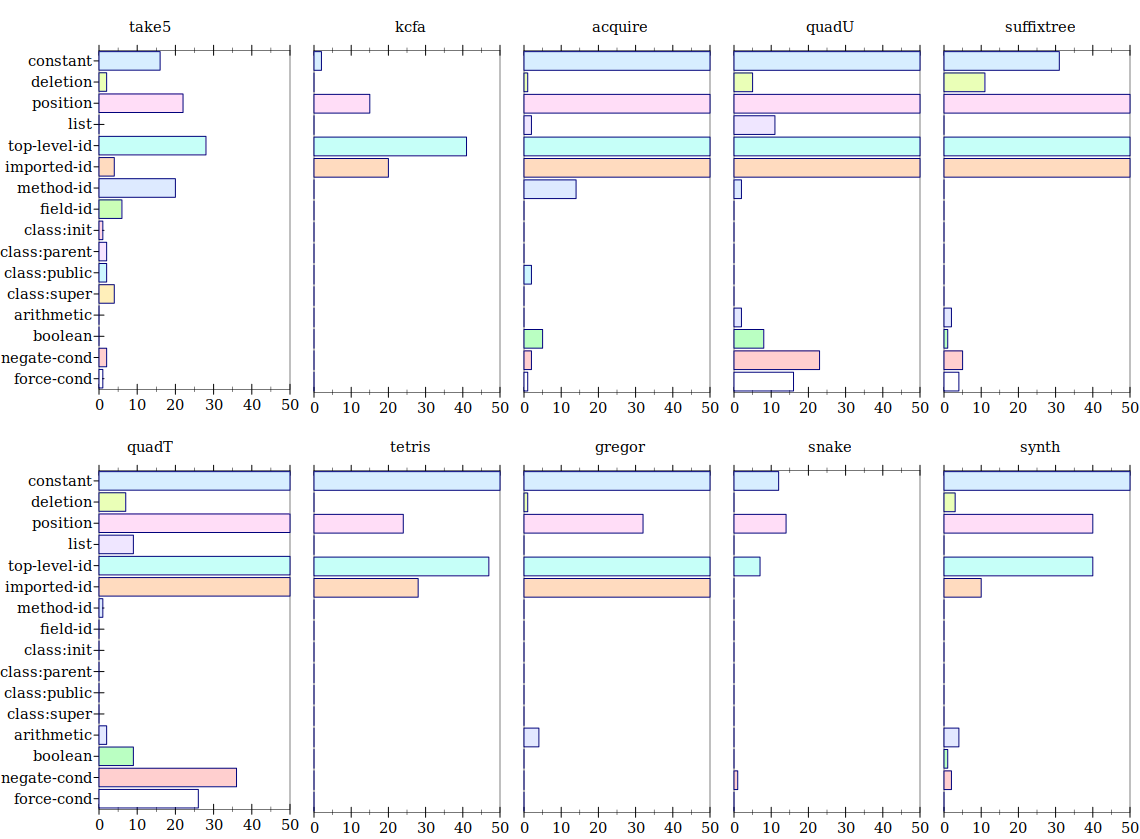
\includegraphics[scale=0.33]{./plots/mutant-breakdown}
  Counts are cut off at 50.

\caption{The mutators produce Interesting debugging scenarios across all benchmarks.} 
 \label{fig:mutant-breakdown}
\end{figure*}

The definition of interesting debugging scenarios creates a powerful filter. All
together, the listed mutators produce 16,800 mutants with at least one
interesting debugging scenario across all benchmarks; see
figure~\ref{fig:mutant-breakdown} for an overview. Broken down by benchmark, the
mutators produce at least 40 interesting scenarios for every benchmark, and
these scenarios originate from at least four different mutators per benchmark.
Thus, the mutators result in a sizable and diverse population of scenarios for
every benchmark.  Furthermore, every mutator contributes scenarios to at least
one benchmark.  Some mutators apply only to a few benchmarks, because they
target rather specific features; for instance, the class-focused mutators are
mainly effective in a program that makes extensive use of object-oriented
features.
